\documentclass[10pt]{article} %indicating type of document, font size
\usepackage[letterpaper, margin=1in]{geometry} %package that allows changes in margins and header/footers
\usepackage{hyperref}
\usepackage[pdftex]{graphicx}  
%\usepackage[leftcaption]{sidecap} %package for adding side captions
\usepackage{sidecap}
\usepackage[labelsep=period]{caption} %package for formatting figure captions, separation between figure number and caption is period
\sidecaptionvpos{figure}{c} %position side caption
\usepackage{lipsum}
\usepackage{indentfirst}
\usepackage{color}
\usepackage{multirow}
\usepackage[document]{ragged2e}
\begin{document}


%\section*{CA Bay Area Sampling Notes}




%Triglochin maritima
%-------------------------------------------------------------------
\begin{SCfigure}
 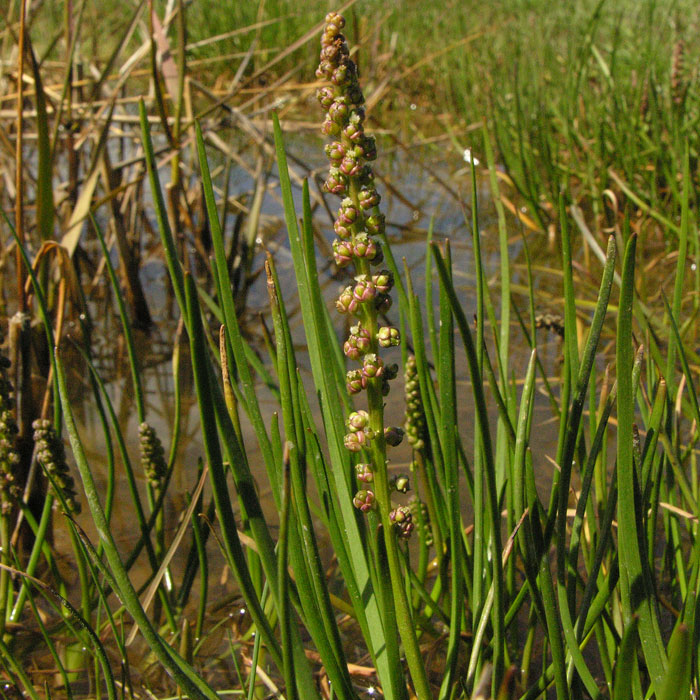
\includegraphics[width=80mm]{Triglochin01.jpg}
 \caption{{\bf{Triglochin maritima, Sea arrowgrass}}\\-In Berkeley Marina, Crissy Field Northern waterfront, Pier 94\\
-Low zone of salt marsh, if high tide will be submerged\\
-narrow rounded leaf blades; 2-3 ft tall\\
-Flower/seed stalks tall, round seeds along stalk; may still have seeds
}
 \end{SCfigure}
%-------------------------------------------------------------------

%Triglochin maritima
%-------------------------------------------------------------------
\begin{SCfigure}
 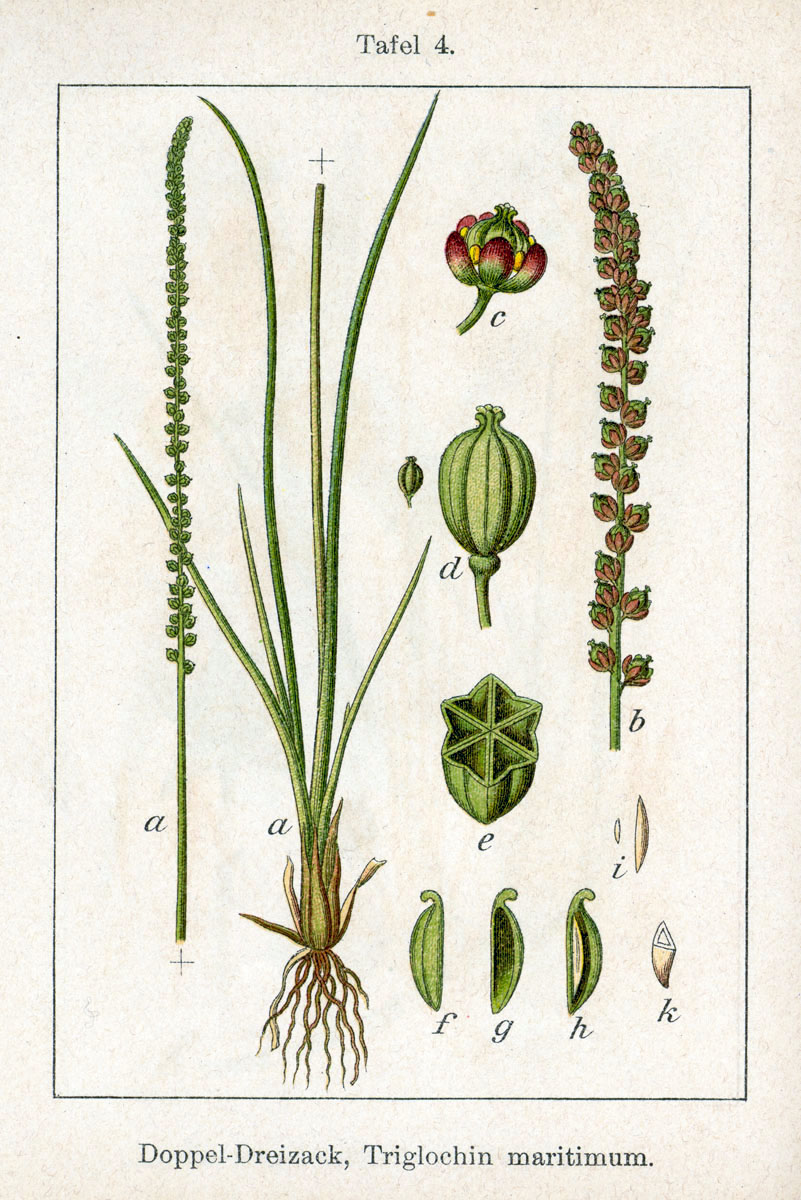
\includegraphics[width=80mm]{Triglochin02.jpg}
 \caption{{\bf{Triglochin maritima, Sea arrowgrass}}\\-In Berkeley Marina, Crissy Field Northern waterfront, Pier 94\\
-Low zone of salt marsh, if high tide will be submerged\\
-narrow rounded leaf blades; 2-3 ft tall\\
-Flower/seed stalks tall, round seeds along stalk; may still have seeds
}
 \end{SCfigure}
%-------------------------------------------------------------------

%Ruppia maritima
%-------------------------------------------------------------------
\begin{SCfigure}
 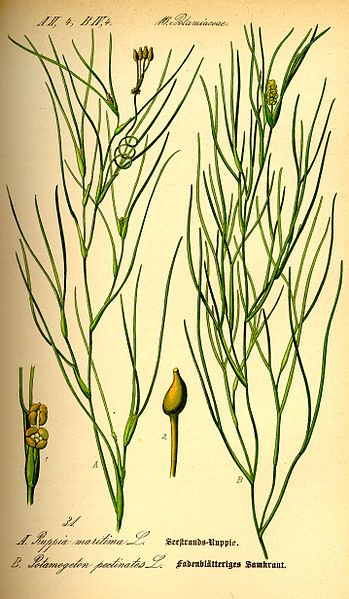
\includegraphics[width=80mm]{Ruppia01.jpg}
 \caption{{\bf{Ruppia maritima; widgeongrass, ditch-grass and tassel pondweed}}\\-Thin threadlike leaves, shallow roots, coiled inflorescence each with 2 flowers; fruits are drupelets\\-Long, narrow, alternate leaves are less than 1 mm wide. Stipular sheaths, less than 7 cm long, are completely fused to the leaf and often broadly clasp the stem\\-Tiny flowers (3-5 mm across), lack petals and sepals, and occur in pairs on stalks. Pollination often occurs underwater or at the waters surface. Once pollinated, the flower stalk coils.\\-Fruits are dark colored, egg to pear-shaped, symmetrical to highly asymmetrical achene is 1.5 to 2 mm long and occurs in a cluster. Each fruit is on individual stalks, but all are connected to a long flowering stalk (peduncle) }
 \end{SCfigure}
%-------------------------------------------------------------------

%Ruppia maritima 02
%-------------------------------------------------------------------
\begin{SCfigure}
 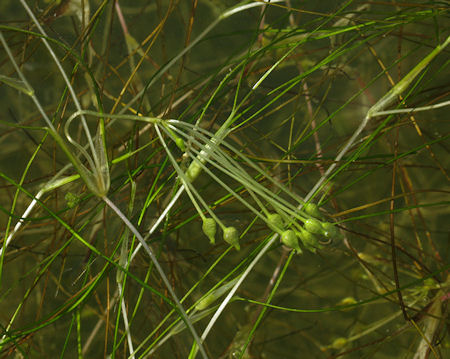
\includegraphics[width=80mm]{Ruppia02.jpg}
 \caption{{\bf{Ruppia maritima; widgeongrass, ditch-grass and tassel pondweed}}\\ -Thin threadlike leaves, shallow roots, coiled inflorescence each with 2 flowers; fruits are drupelets\\-Long, narrow, alternate leaves are less than 1 mm wide. Stipular sheaths, less than 7 cm long, are completely fused to the leaf and often broadly clasp the stem\\-Tiny flowers (3-5 mm across), lack petals and sepals, and occur in pairs on stalks. Pollination often occurs underwater or at the waters surface. Once pollinated, the flower stalk coils.\\-Fruits are dark colored, egg to pear-shaped, symmetrical to highly asymmetrical achene is 1.5 to 2 mm long and occurs in a cluster. Each fruit is on individual stalks, but all are connected to a long flowering stalk (peduncle) }
 \end{SCfigure}
%-------------------------------------------------------------------


\newpage



\end{document}